\documentclass[12pt, a4paper]{article}
\usepackage[tmargin=1.0cm, bmargin=2.5cm, lmargin=2cm, rmargin=2cm]{geometry}
\usepackage[utf8]{inputenc}\DeclareUnicodeCharacter{2212}{-}
\usepackage[T1]{fontenc}
\usepackage{float}
\usepackage{lmodern}
\usepackage{hyperref}
\hypersetup{
colorlinks = true,
linkcolor  = NavyBlue,
citecolor = NavyBlue,
urlcolor = NavyBlue
}
% Bib stuff
\usepackage[
    backend=biber,
    style=apa,
]{biblatex}
\setlength{\bibhang}{0pt}
\setlength{\bibitemsep}{6pt}
\addbibresource[]{../peak_water.bib}
\usepackage{amsmath}
\usepackage{amssymb}
\usepackage{gensymb}
\usepackage{upgreek}
\usepackage{enumitem}
\usepackage{graphicx}
\usepackage{subcaption}
\graphicspath{{../plots/}}
\usepackage[dvipsnames]{xcolor, colortbl}
% Setup for the captions
\usepackage[hypcap=true, labelfont=bf]{caption}
\captionsetup{belowskip=2pt, aboveskip=2pt}

\author{Erik Holmgren \\ Advisor: Fabien Maussion}
\title{Master thesis proposal: Peak water using the Open Global Glacier Model}
\date{March 2021}
\begin{document}
\maketitle
\noindent
\section{Motivation}
Glacier mass loss has increased during the second half of the 20th century
\parencite{vaughanObservationsCryosphere2013} and is predicted, in all current
climate projections, to continue throughout the 21st century
\parencite{ipccClimateChange20142014}. The magnitude of the end of century
glacial mass loss varies greatly depending on the region and climate scenario --
\textcite{hussNewModelGlobal2015} found global glacier volumes to decrease
between 25\% (RCP2.6) and 48\% (RCP8.5) and regional losses varying between 20
and 90\%.

% Simulating global glaciers \textcite{hussNewModelGlobal2015} found that the
% global glacier volume will decrease with 25$\pm$5\% for RCP2.6, 33$\pm$8\% for
% RCP4.5 and 48$\pm$9\% by the end of the century. Furthermore, they found large
% regional differences -- glaciers in central Europe and in low latitudes may lose
% as much as 90\% of their mass while glaciers in Arctic Canada and
% Antarctica/Subantarcitca lose 20\%. 

% End of century glacier mass exhibit a substantial spread depending on the GCM
% used for the emission scenario in the simulation. For instance, mass losses in
% Svalbard varies between 12\% and 90\% for RCP4.5
% \parencite{hussNewModelGlobal2015}.

Glaciers play an important role as a form of water storage, delaying up to 79\%
of the total precipitation falling on the glacier surface (Aral Basin) through
the release of meltwater during the ablation season. Benefits of this seasonal
delay is particularly important in regions with a warm and dry ablation season
\parencite{kaserContributionPotentialGlaciers2010}. One of those areas is the
Indus basin where, during the pre-monsoon season, up to 60\% of the total
irrigation volume comes from either snow or glacier melt -- resulting in an 11\%
increase of the total crop production
\parencite{biemansImportanceSnowGlacier2019}. Simultaneously, the Indus basin is
an example of a large river basin which under the present climate experiences
water scarcity -- threatening the food security of millions of people
\parencite{kummuClimatedrivenInterannualVariability2014}. This in an area where
large amounts of the freshwater resource is shared across state borders where
the risk for armed conflict is high
\parencite{schleussnerArmedconflictRisksEnhanced2016,
pritchardAsiaShrinkingGlaciers2019}. 

The populated areas on the dry, western, slopes of the Andes are other examples
of regions depending on glacier meltwater for potable water and power
generation. \textcite{vergaraEconomicImpactsRapid2007} estimate the cost of
mitigation and adaption to retreating glaciers in the Andes to between US\$300
million and US\$ 1.5 billion.

Maybe something on Europe? But no real scarcity here?
% of glacier melt include significant contributions to sea level rise (e.g.
% \cite{marzeionFutureSealevelChange2012a})

% More direct societal impacts The Indus basin is experiencing water scarcity under the present climate
% \parencite{kummuClimatedrivenInterannualVariability2014}.

% Out of the total precipitation falling onto the glacier surface, between 79 and
% 17\% will experience a seasonal delay -- meaning that the water will be stored
% in the glacier and released later in the season. The relative importance of
% glacier melt water to the basin water availability decreases in the presence of
% liquid precipitation, hence the positive effects of seasonally delayed water
% release from glaciers are more pronounced in areas experiencing warm and dry
% ablation seasons \parencite{kaserContributionPotentialGlaciers2010}.

% The monthly percentage of total water input to a basin that experience seasonal
% delayed water release by glaciers decreases downstream the river while the
% population generally increases. Thus, the societal impacts of seasonal delayed
% water release by glacier melt reaches a maximum at intermediate altitude bands
% \parencite{kaserContributionPotentialGlaciers2010}.

\section{State of the art -- Glacial hydrology}
Glaciers store water in multiple ways -- as a liquid in surface snow and firn,
in crevasses, drainage networks, englacial pockets and surface pools, or as a
solid in the form of snow, firn and ice
\parencite{janssonConceptGlacierStorage2003}. The main factors controlling the
discharge hydrograph of an Alpine basin is the topographical structure, the
seasonal air temperature gradient, the seasonal distribution of precipitation
\parencite{zappaSeasonalWaterBalance2003}, and the percentage of glaciated area
within the basin \parencite{janssonConceptGlacierStorage2003}. 

Melt is the process with the largest contribution to glacier runoff, resulting
in that the fraction of summer runoff to the annual runoff increases with an
increased glaciation
\parencite{zappaSeasonalWaterBalance2003,chenInfluenceAlpineGlaciers1990}.
Furthermore, \textcite{blissGlobalResponseGlacier2014} showed that glacier net
mass loss is an important part of the total glacier runoff, indicating that the
societal importance of glacier melt water might be higher than the estimates
from \textcite{kaserContributionPotentialGlaciers2010}, where runoff estimates
were done under an assumed equilibrium.
% Glacier runoff peaks late in the summer -- when the melt line has crept further
% up and thus exposing more of the catchment area to melt
% \parencite{zappaSeasonalWaterBalance2003}.

% In alpine catchments snow accumulation and snow melt are the main contributors
% to runoff generation, while the influence of precipitation is small, during the
% months between June and October \parencite{zappaSeasonalWaterBalance2003}. 

% The estimated the societal importance of glacier melt water from
% \textcite{kaserContributionPotentialGlaciers2010} was made under the assumption
% that the glaciers were in equilibrium with the local climate -- i.e. none of the
% runoff estimations included any net mass loss.

The term `peak water` is an adaption of the more well known term \emph{Peak Oil}
-- which indicates the period in time when production of oil reaches a maximum,
after which it begin to decrease \parencite{gleickPeakWaterLimits2010}. Recently
this term has been applied to meltwater generation from glaciers (e.g.
\cite{hussGlobalscaleHydrologicalResponse2018}) as a way to put the impacts of
shrinking glaciers into a societal context. The mechanism behind glacial peak
water is fairly straight forward: When climate change causes a glacier to
recede, water is released from long term glacial storage and the annual runoff
will increase until a maximum is reached i.e. peak water. At this point and
forward the annual runoff will begin to decrease since the area of the shrinking
glacier is not able to produce the same amounts of meltwater any longer
\parencite{janssonConceptGlacierStorage2003}. If the glacier reaches a new state
of equilibrium (zero net mass loss), the annual runoff from the initially
glaciated area can return to pre peak water levels. However, runoff levels
during the melt season can be expected to fall below the pre peak water levels
since melt water from long term storage will be reduced 
\parencite{hussGlobalscaleHydrologicalResponse2018,
ragettliContrastingClimateChange2016, immerzeelRisingRiverFlows2013} (see Fig.
\ref{fig:peak_water}) (This citation needs some work). 
\begin{figure}[h]
    \centering
    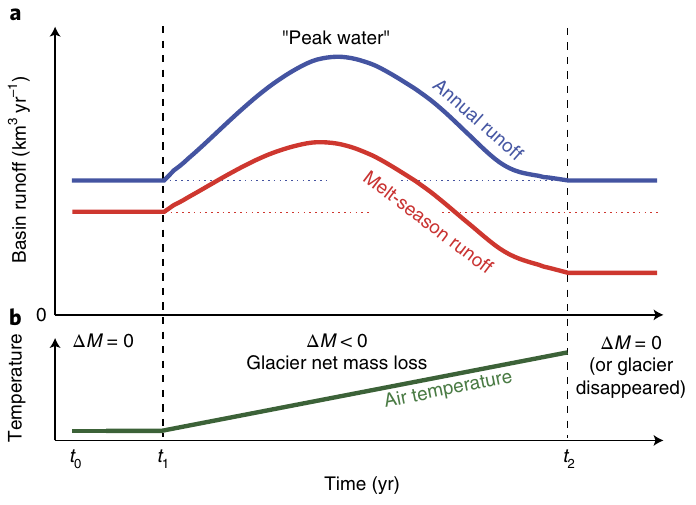
\includegraphics[width=0.6\textwidth]{../peak_water.png}
    \caption{Schematised view of glacier runoff and peak water during a
    transient state. The annual glacier runoff will be constant from year to
    year during equilibrium. If the conditions change so that the glacier is no
    longer in equilibrium with its climate and the glacier begins to loose mass,
    the melt season runoff will increase with rising temperatures.
    Borrowed from \textcite{hussGlobalscaleHydrologicalResponse2018}.}
    \label{fig:peak_water}
\end{figure}

\section{Peak water using the Open Global Glacier Model}
State of the art peak water estimations (e.g.
\cite{rounceGlacierMassChange2020,hussGlobalscaleHydrologicalResponse2018}) have
relied on parametrizing the re-distribution of mass throughout the glacier with
so called mass re-distribution curves, developed by
\textcite{hussFutureHighmountainHydrology2010}. This parameterization is a clear
step up in performance compared to previous ice flow parametrizations (e.g.
length-area scaling), but still relies on multiple DEMs covering the glacier for
calibration of the flow as a function of the mass balance. As a consequence, the
flow, or mass re-distribution, of non-measured glaciers will be estimated from
known glaciers of a similar size not considering topographical differences. 

Employing the Open Global Glacier Model (OGGM,
\cite{maussionOpenGlobalGlacier2019}) for peak water calculations would be the
first time a physical ice flow model is applied globally to calculate glacier
runoff. It would be a step towards mitigating the problem of over
parametrization present in the current global glacier models used for
hydrological analysis. Including ice dynamics in global glacier simulations
result in reduced ice losses compared to parametrized models
\parencite{zekollariModellingFutureEvolution2019}, possibly resulting in
more accurate runoff estimations. The inclusion of ice dynamics also enables the
glacier to grow, if climatic conditions allow it, and not only to shrink -- a
limitation of parametrized ice dynamics. Using the OGGM will thus provide a new
view of global glacier runoff and peak water estimations, expanding the
grasp of the subject.

% A new set of runoff estimates, based on a different modelling framework, will
% broaden the scientific background about the subject. The OGGM uses the same
% mass balance scheme, a degree day model, as for example PyGEM (used by
% \cite{rounceGlacierMassChange2020}). Thus, any differences in the annual mass
% balance should stem from the different implementations of ice dynamics --
% possibly leading to slightly different area/length estimations and thus a
% different runoff.

In its current state the OGGM does not calculate any hydrological outputs for
the glaciers (not true any more...). This has to be implemented before any
runoff simulations. The common approach is to use a so called fixed gauge -- a
hypothetical measuring station at the terminus of the glacier, measuring all
water leaving the initially glaciated area. Runoff, $Q$, is calculated from the
ablation $\alpha$, the liquid precipitation $p_{liquid}$, and the refreezing
of meltwater within the glacier $R$ as:
\begin{equation}
    Q = \alpha + p_{liquid} - R.
\end{equation}
The contribution from ablation is made up of ice and snow melt, which can be
estimated from the excess melt water of the glacier. This is where it becomes a
bit tricky. Excess meltwater is produced during years with a negative mass
balance, but since this can vary from year to year excess meltwater has to be
calculated retroactively for each mass-balance year. This process starts with
calculating the total excess meltwater for the period in question (i.e. net mass
change). This can then be distributed, sequentially, to all negative
mass-balance year where mass is not regained in the future
\parencite{rounceGlacierMassChange2020}. Runoff originating from snow melt and
liquid precipitation is measured from the initially glaciated area. As the
glaciated area shrinks, this fraction of the runoff is divided into two parts:
on glacier runoff and off glacier runoff. The OGGM does not parametrize
refreezing, and instead relies on the calibration of the mass balance model to
compensate for this.


\subsection{Research questions}
For this thesis I will try to answer the following questions:
\begin{enumerate}
    \item \textbf{How does the inclusion of ice dynamics in a global glacier
    model change the future temporal and spatial variation of peak water?}
    The inclusion of ice dynamics will results in a different annual mass
    balance compared to models relying on parametrization. Since the runoff
    estimations are based on the mass balance -- any changes to its calculation
    should result in a different estimate of peak water.
    \item \textbf{High mountain Asia, when will the basins most dependent on
    glacier runoff reach peak water?} This would basically be done to
    corroborate on the previous studies that have been done. The \textbf{Indus
    basin}.
    \item \textbf{At which levels, and during what time, will runoff levels
    begin to stabilise again?} Peak water gives a measure of when the annual
    runoff from glaciers reaches a maximum, but what about the long term
    equilibrium? What will the future water supply look like?
    \item \textbf{How will the seasonal hydrograph change for future runoff
    projections?} Will glaciers release water earlier in the season? Or later?
    Also connects to the previous question -- how is the annual runoff affected?
\end{enumerate}

\section{Schedule or something}
Hydrological outputs were recently implemented in the OGGM, but still need to be
evaluated and fully integrated into the model. To make sure that this is doing
what is intended is the first step of this work. This include testing the
implementation, running a few simulations on a smaller scale and document it.
Based on results from previous studies, a number of regions interesting in
regards to peak water can be selected for long term simulations using the OGGM.
To evaluate the affect of ice dynamics on glacier runoff the results can then
be compared to previous studies. A regional analysis is a natural continuation
of this -- Take a look at the Indus basin.

Evaluating future stabilised levels requires the glaciers to have reached a new
equilibrium. If, and when, glaciers will reach a new equilibrium is kind of an
open question and would require to run the simulation for 100s of years. So not
actually sure if this will be possible.

The seasonal hydrology will be analysed in conjunction with the regional
analysis of one or two regions where the global simulations showed interesting
results in terms of peak water.




\printbibliography
\end{document}